\documentclass{article}

\usepackage[dutch]{babel}
\usepackage{hyperref}
\usepackage{graphicx}
\usepackage{standalone}
\usepackage{pdfpages}

% style
\setlength{\parindent}{0pt}
\usepackage[left=2.5cm,top=2cm,right=2.5cm,bottom=2cm,a4paper]{geometry}
\usepackage{fancyhdr}
\pagestyle{fancy}
\lhead{Team 6}
\renewcommand{\headrulewidth}{0.4pt}

\begin{document}
	\section*{Samenvatting klantenvereisten}
	Budget: 
	\begin{itemize}
		\item 3500 eenheden
	\end{itemize}
	Wat het miniatuurrobotwagentje moet kunnen: 
	\begin{itemize}
		\item Het moeten lijnen van heldere plakband (met lengte 1 meter en breedte 25 millimeter) volgen die straten voorstellen in een modelstad.
		\item Het moet andere robotwagentjes detecteren als ze voor hun rijden, om zo botsingen te vermijden.
		\item De wagen moet verkeerslichten interpreteren op een hoogte van 7,5 centimeter. Daarmee bedoelt men dat wanneer het rood is, het wagentje stopt. Als het groen licht is, moet de wagen doorrijden of afslaan.
		\item Het robotwagentje moet lijnsoorten interpreteren
		\subitem Wanneer hij een volglijn detecteert, zal hij rijden. Dit is wanneer de lijn dezelfde richting staat als de wagen.
		\subitem Bij een stoplijn, zal hij stoppen. Dit is het geval aan een kruispunt en bij verkeerslichten. Deze lijn staat dwars op de auto en is 50 millimeter breed.
		\item Bij het rijden moet het een aanvaardbare snelheid hebben zodat het verkeer niet wordt opgehouden.
		\subitem Het moet snel kunnen stoppen als de stopstreep gedetecteerd wordt (minder dan 10cm/s).
		\subitem Het autootje mag niet te lang over het traject doen (sneller dan 1cm/s).
		\item De wagen moet bestuurbaar zijn vanop een afstand om het bijvoorbeeld tijdens het traject te kunnen overnemen.
	\end{itemize}
	
	% NOTE: Alle bestandslocaties zijn aangepast naar hun eigen
	
	% overzicht van de ontwerpspecificaties
	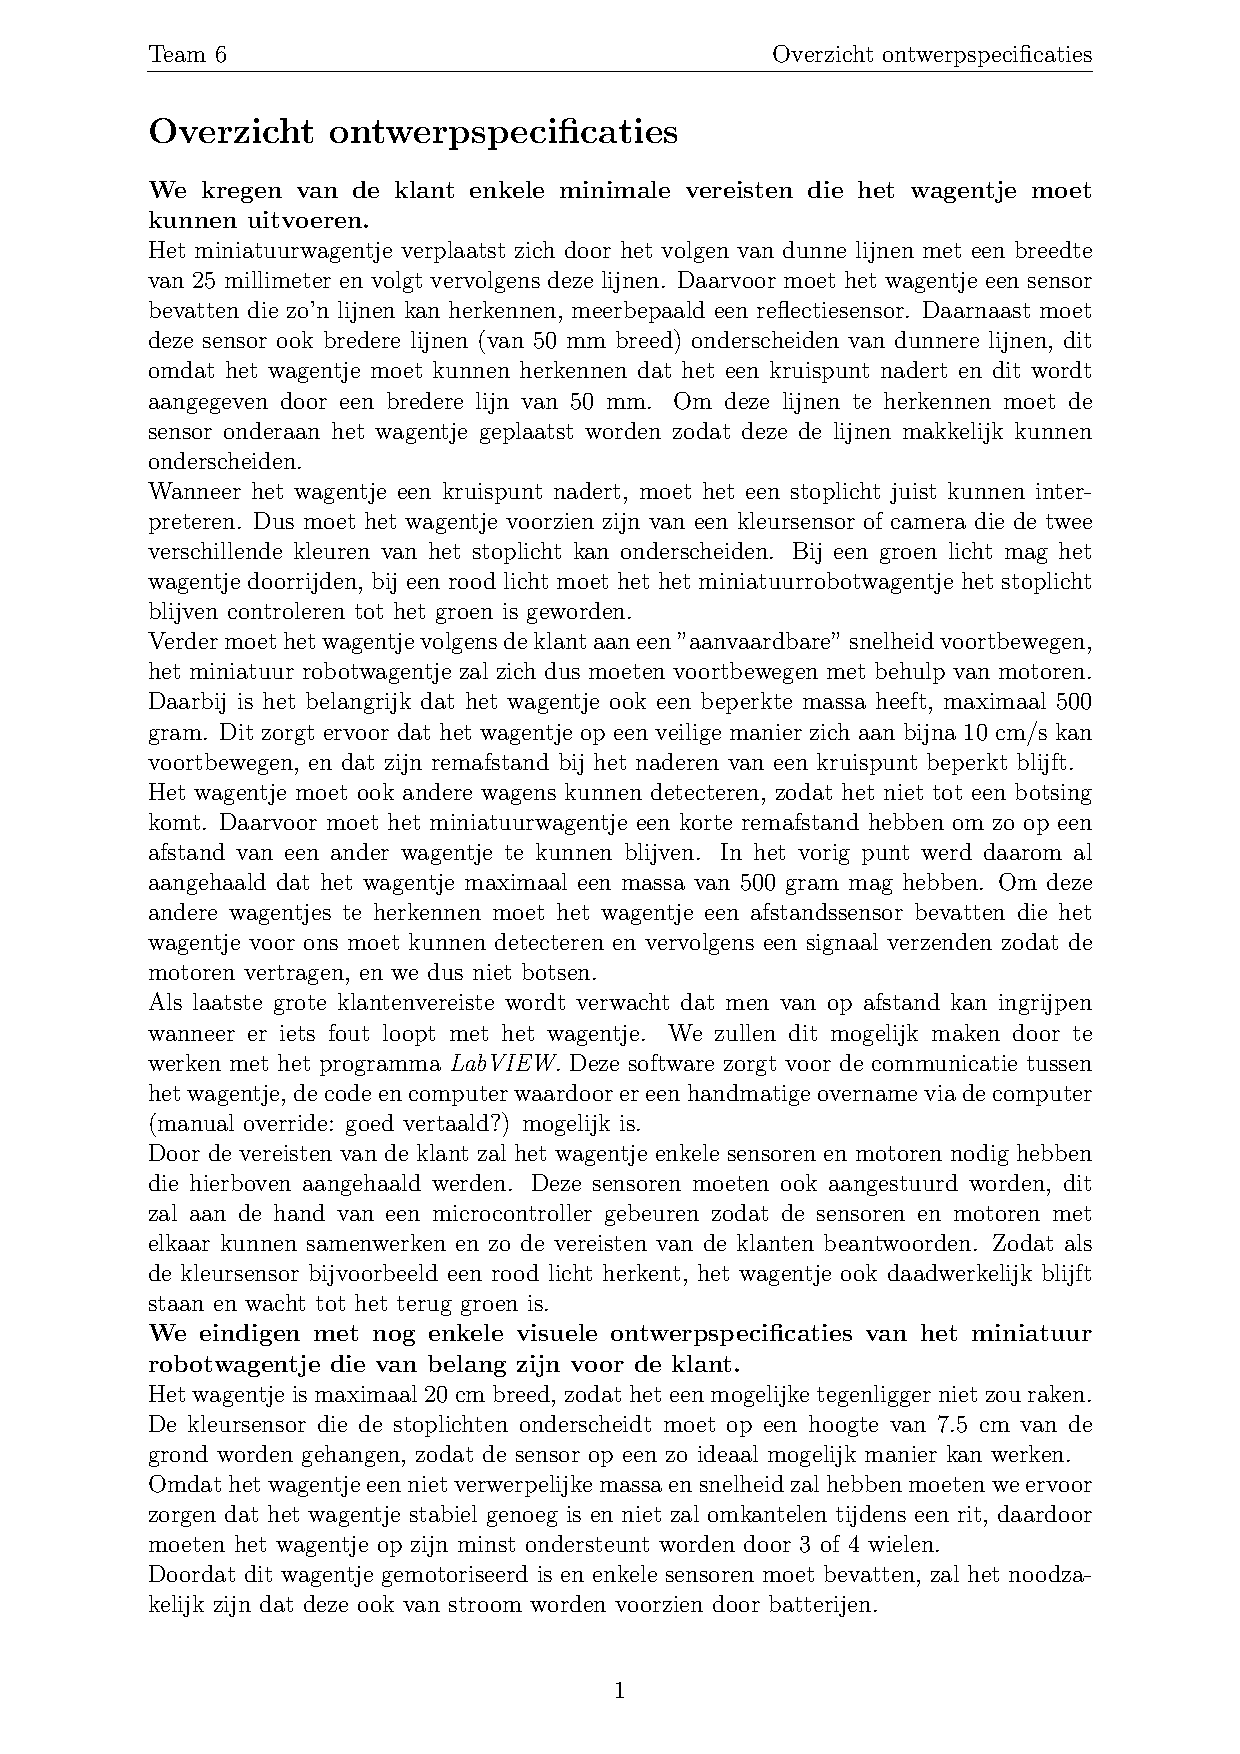
\includepdf[pages=-]{ontwerpspecificaties/ontwerpspecificaties.pdf}
	
	%\section*{Takenstructuur} % nog niet mooi weergegeven
	
\includepdf[pages=-]{taakstructuur/taakstructuur.pdf}
	
	%\section*{Verantwoordelijkheidsstructuur}
	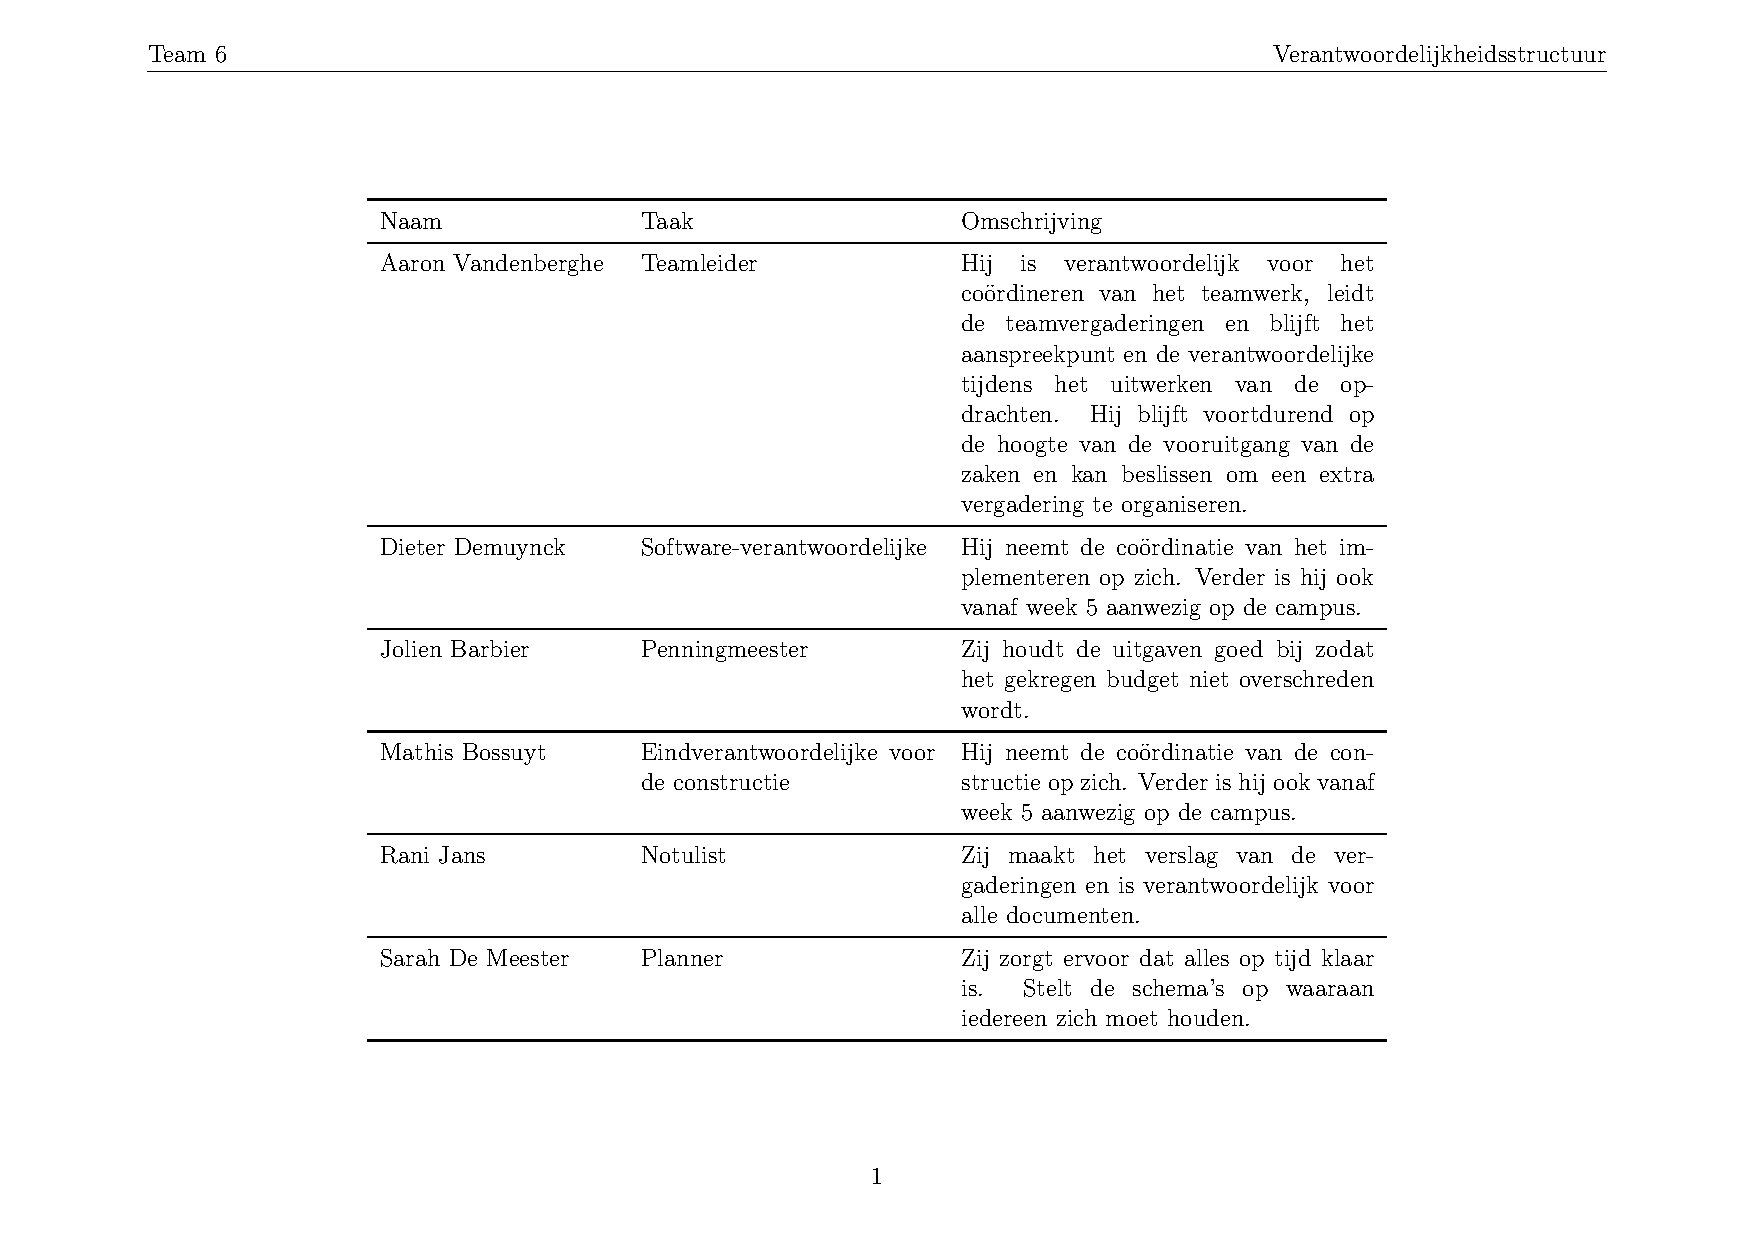
\includepdf[pages=-]{verantwoordelijkheidsstructuur/verantwoordelijkheidsstructuur.pdf}
	
	% teamkalender
	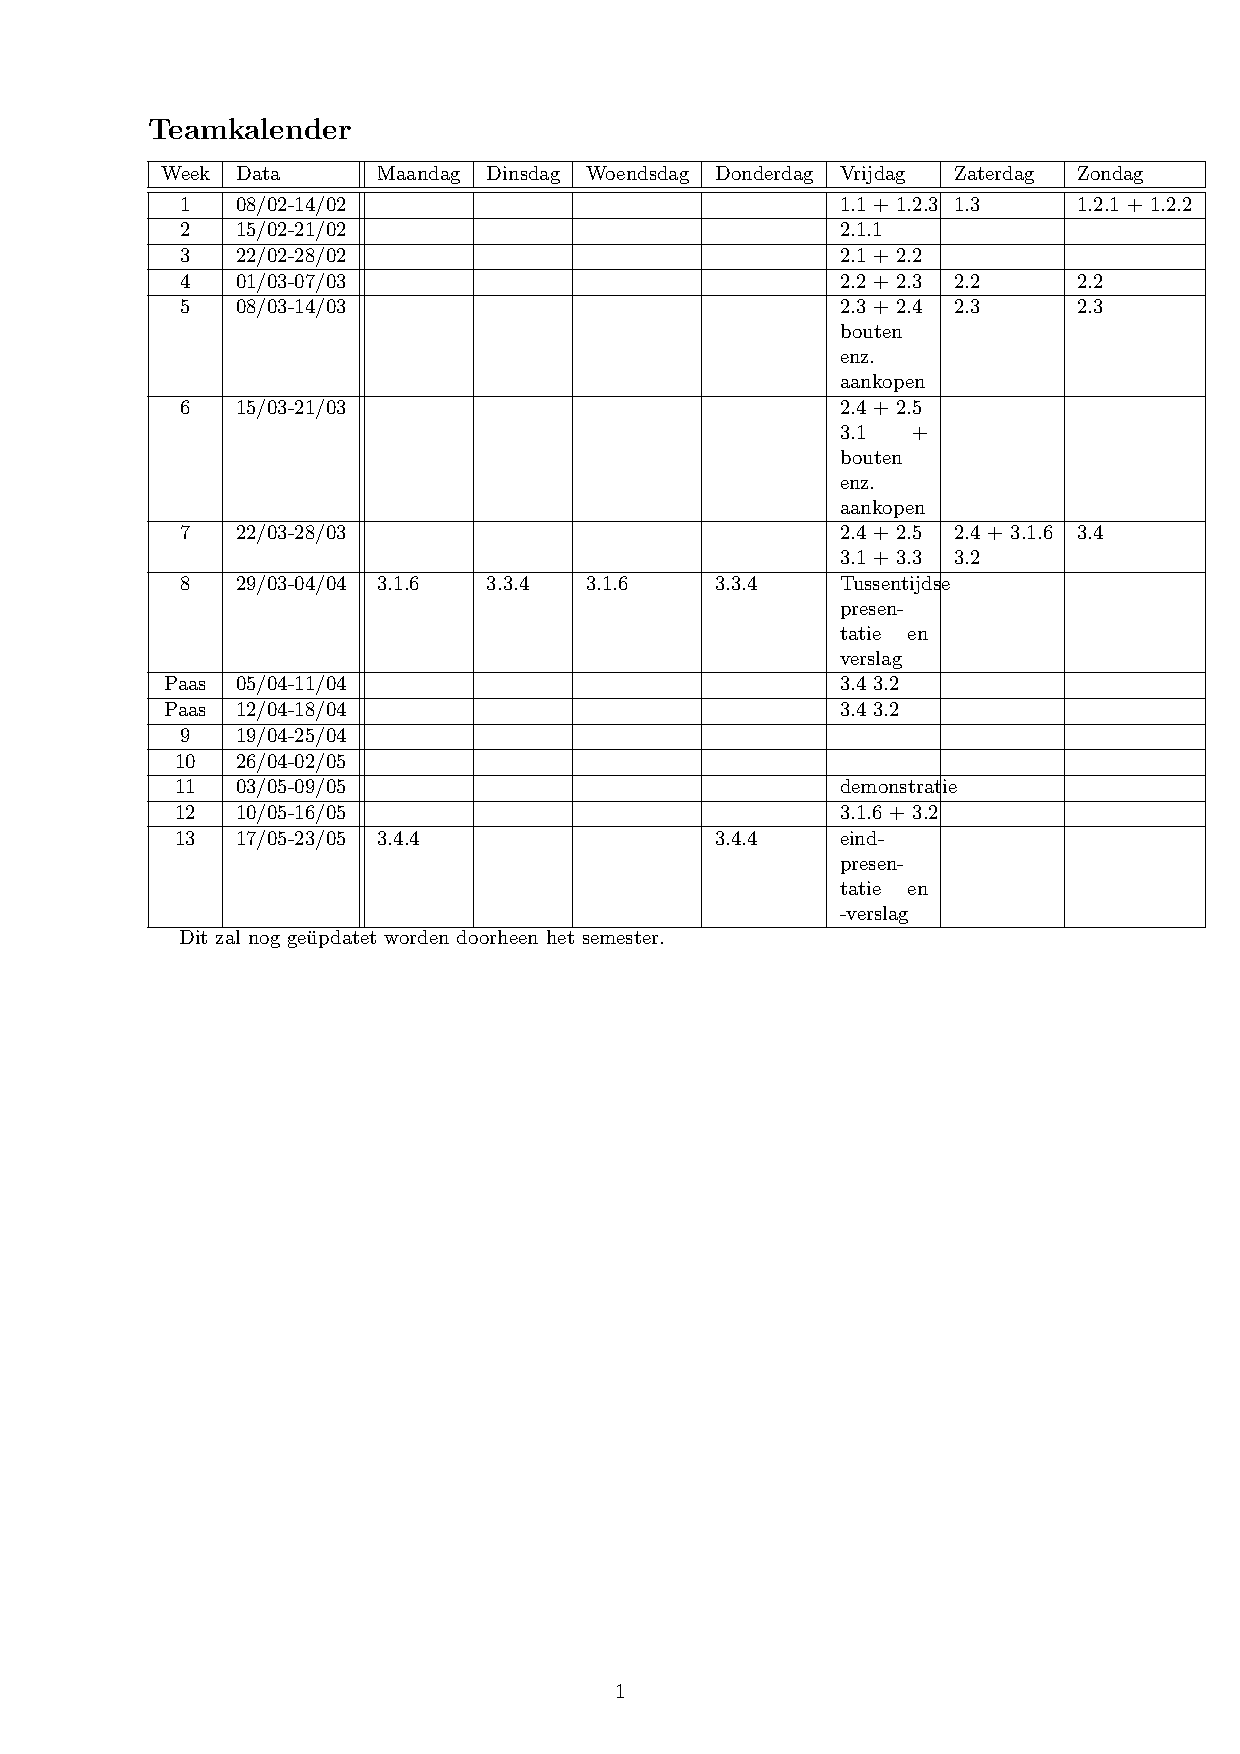
\includepdf[pages=-]{team6kalender/team6kalender.pdf}
	
	%\section*{Gannt-chart}	%nog niet mooi weergegeven
	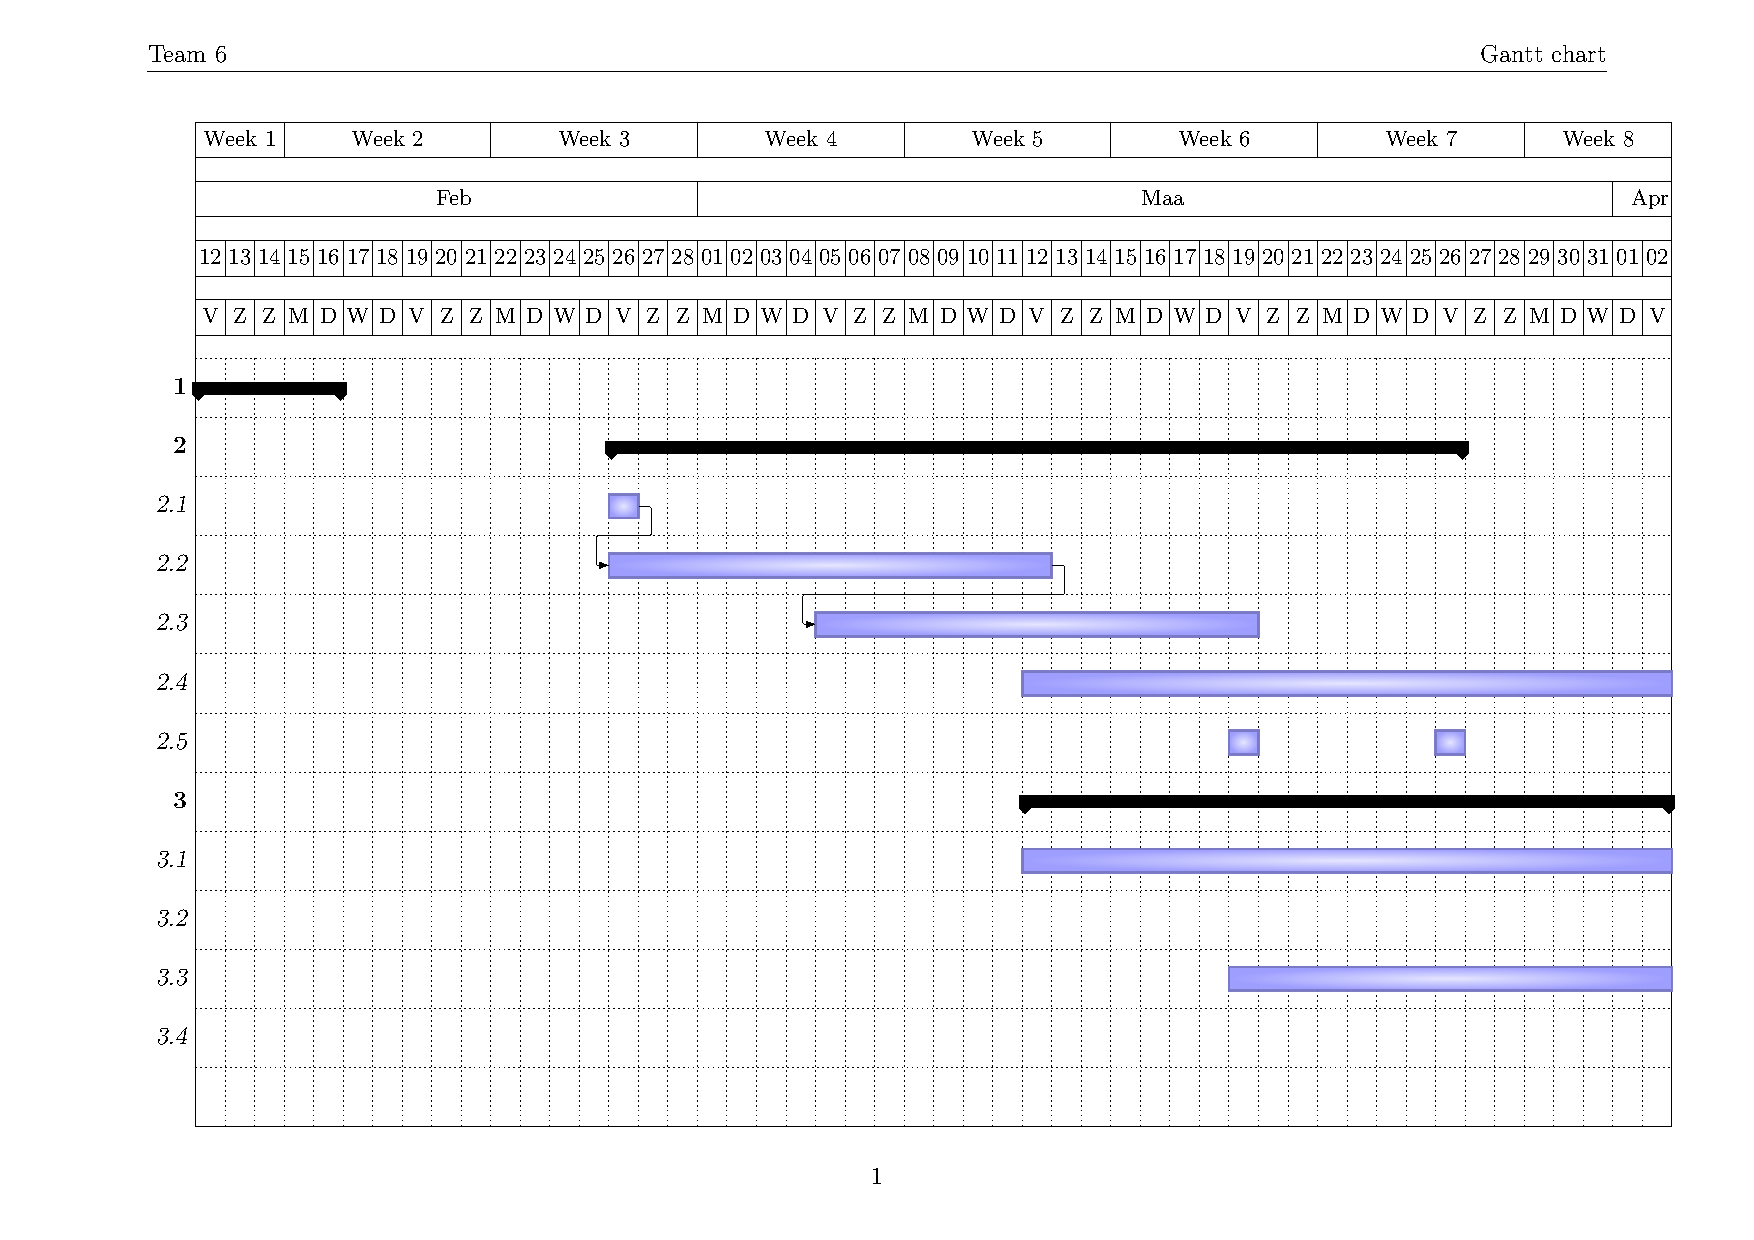
\includepdf[pages=-]{ganttchart/ganttchart.pdf}
\end{document}
